\documentclass[aspectratio=169,10pt]{beamer}

\usetheme{Madrid}
\usecolortheme{seahorse}

\usepackage{amsmath,amssymb}
\usepackage{booktabs}
\usepackage{array}
\usepackage{graphicx}
\usepackage{ragged2e}
\usepackage{tabularx}
\usepackage{tikz}
\usepackage{pgfplots}
\usepackage{iftex}
\pgfplotsset{compat=1.18}

\ifPDFTeX
  \pdfmapfile{+cm.map}
  \pdfmapfile{+cmextra.map}
  \pdfmapfile{+symbols.map}
\fi

\definecolor{CourseBlue}{RGB}{41,77,115}
\definecolor{CourseGreen}{RGB}{63,125,88}
\definecolor{CourseGold}{RGB}{190,137,45}
\definecolor{CourseRed}{RGB}{169,75,70}
\definecolor{SoftGrid}{RGB}{218,225,232}
\definecolor{CodeBack}{RGB}{245,247,249}

\setbeamercolor{structure}{fg=CourseBlue}
\setbeamertemplate{navigation symbols}{}
\setbeamertemplate{itemize items}[circle]
\setbeamertemplate{enumerate items}[default]

\title[Chapter 18: Comparing Two Means]{\textbf{Chapter 18: Comparing Two Means}}
\subtitle{The Practice of Statistics in the Life Sciences \\ Brigitte Baldi and David S. Moore}
\author{Instructor: Ali Raisolsadat}
\date{Part IV: Specific Inference Procedures}

\begin{document}

% =============================================================
% INTRODUCTION AND STUDY DESIGN
% =============================================================

% SLIDE 1
\begin{frame}
  \titlepage
\end{frame}

% SLIDE 2
\begin{frame}{Why Chapter 18 Matters}
Chapter 17 developed inference for one population mean and for paired differences.

\vspace{0.25cm}
Many scientific questions instead compare two separate populations or two independent treatment groups.

\begin{block}{Main Question}
How can two independent samples be used to estimate or test the difference between two population means?
\end{block}

The main parameter is now a difference, $\mu_1-\mu_2$, rather than a single mean.
\end{frame}

% SLIDE 3
\begin{frame}{Chapter Roadmap}
The chapter develops the following connected ideas.

\begin{enumerate}
  \item Recognize independent two-sample problems
  \item Describe two groups before performing inference
  \item Derive the standard error of $\bar{x}_1-\bar{x}_2$
  \item Construct Welch two-sample $t$ intervals and tests
  \item Assess robustness to non-Normality
  \item Understand why pooled procedures and inference about standard deviations require caution
\end{enumerate}

The reasoning is the same as in earlier chapters: study design first, then conditions, calculation and interpretation.
\end{frame}

% SLIDE 4
\begin{frame}{What Is a Two-Sample Problem?}
A two-sample problem compares a quantitative response across two distinct groups.

\begin{itemize}
  \item There is one sample from each population or treatment group
  \item The same quantitative response is measured in both groups
  \item The individuals in one sample are unrelated to those in the other sample
  \item The two sample sizes may be different
\end{itemize}

\begin{block}{Goal}
Estimate or test the difference between the population means, $\mu_1-\mu_2$.
\end{block}
\end{frame}

% SLIDE 5
\begin{frame}{How Two Independent Samples Arise}
Two-sample data can come from several designs.

\begin{itemize}
  \item \textbf{Randomized experiment:} Experimental units are randomly assigned to two treatments
  \item \textbf{Separate random samples:} One random sample is selected from each of two populations
  \item \textbf{Subgroups of one sample:} A random sample is divided using a pre-existing characteristic such as species, habitat or sex
\end{itemize}

The design determines whether the comparison can support a causal conclusion, a population generalization, both or neither.
\end{frame}

% SLIDE 6
\begin{frame}{Independent Samples or Matched Pairs?}
The correct procedure depends on how the observations were produced.

\begin{center}
\begin{tabularx}{0.94\textwidth}{>{\RaggedRight\arraybackslash}p{0.20\textwidth} X X}
\toprule
 & \textbf{Independent samples} & \textbf{Matched pairs} \\
\midrule
Relationship & Different, unrelated individuals & Same individual twice or deliberately matched units \\
Analysis & Compare $\bar{x}_1-\bar{x}_2$ & Calculate paired differences first \\
Procedure & Two-sample $t$ & One-sample $t$ on differences \\
Example & Two separate chicken groups & Before-and-after blood pressure \\
\bottomrule
\end{tabularx}
\end{center}

Ignoring a real pairing discards information. Inventing a pairing between unrelated observations is also incorrect.
\end{frame}

% SLIDE 7
\begin{frame}{What Conclusions Does the Design Support?}
\begin{center}
\begin{tabularx}{0.95\textwidth}{>{\RaggedRight\arraybackslash}p{0.29\textwidth} X X}
\toprule
\textbf{Design feature} & \textbf{What it supports} & \textbf{What it does not guarantee} \\
\midrule
Random sampling & Generalization to the sampled population & Causation \\
Random assignment & Causal comparison of treatments & Generalization beyond the experimental units \\
Both & Causal inference and population generalization & Protection from noncompliance or measurement problems \\
Neither & Association in the observed data & Broad generalization or causation \\
\bottomrule
\end{tabularx}
\end{center}

A small $P$-value cannot compensate for a weak study design.
\end{frame}

% SLIDE 8
\begin{frame}{A Quantitative Response and a Two-Level Factor}
A two-sample problem can be viewed as a bivariate problem.

\begin{itemize}
  \item The \textbf{response variable} is quantitative
  \item The \textbf{explanatory variable} is categorical with two levels
\end{itemize}

\begin{block}{Example}
In a study of a feed supplement and calf growth, weight gain is the quantitative response and supplement status (supplement or control) is the two-level factor.
\end{block}

The statistical question concerns the difference between the two population mean responses.
\end{frame}

% SLIDE 9
\begin{frame}{Examples of Two-Sample Questions}
\small
\begin{center}
\begin{tabularx}{0.95\textwidth}{>{\RaggedRight\arraybackslash}p{0.34\textwidth} X X}
\toprule
\textbf{Study} & \textbf{Response} & \textbf{Two groups} \\
\midrule
Triclosan exposure in mice & Liver weight & Triclosan diet; control diet \\
Young chimpanzee behaviour & Time in contact with mother & Male; female \\
Pertussis records & Time since vaccination & Diagnosed; not diagnosed \\
Transgenic chickens & Hatching weight & Transgenic; commercial \\
\bottomrule
\end{tabularx}
\end{center}

In every case, the same quantitative variable is compared across two independent groups.
\end{frame}

% =============================================================
% CONDITIONS AND THEORY
% =============================================================

\section{Conditions and Theory}

% SLIDE 10
\begin{frame}{Describe the Data Before Inference}
Begin with side-by-side graphs and numerical summaries.

\begin{itemize}
  \item Use dotplots for small samples
  \item Use boxplots or histograms for larger samples
  \item Compare shapes, centres and spreads
  \item Look for skewness, clusters, gaps and outliers
  \item Check whether a mean is scientifically meaningful for each group
\end{itemize}

\begin{block}{Why This Comes First}
The two-sample $t$ procedure summarizes a difference in means. A graph can reveal features that the two means cannot describe.
\end{block}
\end{frame}

% SLIDE 11
\begin{frame}{Conditions for Comparing Two Means}
Welch two-sample $t$ procedures rely on three main ideas.

\begin{enumerate}
  \item Each sample represents its population or treatment group through a defensible random process
  \item The two samples are independent of one another
  \item Each population is Normal, or the samples are large enough for the procedure to be reliable without strong outliers
\end{enumerate}

The two population means and standard deviations are unknown. Equal population variances are \textbf{not} required.
\end{frame}

% SLIDE 12
\begin{frame}{Independence Has Two Levels}
The design should support independence both within and between samples.

\begin{itemize}
  \item \textbf{Within a sample:} One observation should not determine another
  \item \textbf{Between samples:} An individual in Group 1 should not be paired or otherwise linked with an individual in Group 2
  \item When sampling without replacement, each population should be much larger than its sample
\end{itemize}

\begin{block}{Common Violation}
Measurements taken before and after treatment on the same animals are paired, not independent. They require a matched pairs analysis.
\end{block}
\end{frame}

% SLIDE 13
\begin{frame}{Shape, Outliers and Sample Size}
The reliability of the procedure depends on both groups.

\begin{itemize}
  \item With small samples, each distribution should be reasonably symmetric and free of outliers
  \item Moderate samples can tolerate mild skewness
  \item Larger samples can tolerate more skewness because of the Central Limit Theorem
  \item Extreme outliers can strongly affect a sample mean and standard deviation even when the other group is well behaved
\end{itemize}

Assess the two distributions separately. One acceptable graph does not repair a serious problem in the other group.
\end{frame}

% SLIDE 14
\begin{frame}{Population Notation}
Each group has its own population mean and standard deviation.

\begin{center}
\begin{tabular}{cccc}
\toprule
\textbf{Population} & \textbf{Variable} & \textbf{Mean} & \textbf{Standard deviation} \\
\midrule
1 & $X_1$ & $\mu_1$ & $\sigma_1$ \\
2 & $X_2$ & $\mu_2$ & $\sigma_2$ \\
\bottomrule
\end{tabular}
\end{center}

\begin{block}{Parameter of Interest}
The population difference is $\mu_1-\mu_2$. Its sign depends on which group is labelled Group 1.
\end{block}

Define the order before calculating or interpreting the difference.
\end{frame}

% SLIDE 15
\begin{frame}{Sample Notation}
The two samples provide estimates of the four unknown population quantities.

\begin{center}
\begin{tabular}{cccc}
\toprule
\textbf{Sample} & \textbf{Size} & \textbf{Mean} & \textbf{Standard deviation} \\
\midrule
1 & $n_1$ & $\bar{x}_1$ & $s_1$ \\
2 & $n_2$ & $\bar{x}_2$ & $s_2$ \\
\bottomrule
\end{tabular}
\end{center}

The natural estimate of $\mu_1-\mu_2$ is
\[
\bar{x}_1-\bar{x}_2
\]

This estimate is unbiased when the samples are produced by appropriate random processes.
\end{frame}

% SLIDE 16
\begin{frame}{The Difference Must Keep Its Order}
Suppose Group 1 is the treatment group and Group 2 is the control group.

\[
\text{estimated treatment effect}=\bar{x}_1-\bar{x}_2
\]

\begin{itemize}
  \item A positive value means the treatment sample mean is larger
  \item A negative value means the treatment sample mean is smaller
  \item Reversing the group labels reverses the sign but not the strength of the evidence
\end{itemize}

State the subtraction order in words before interpreting an interval or test statistic.
\end{frame}

% SLIDE 17
\begin{frame}{Centre of the Sampling Distribution}
Across repeated independent samples,

\[
E(\bar{X}_1)=\mu_1
\qquad\text{and}\qquad
E(\bar{X}_2)=\mu_2
\]

Therefore,

\[
E(\bar{X}_1-\bar{X}_2)=\mu_1-\mu_2
\]

\begin{block}{Interpretation}
The difference in sample means is an unbiased estimator of the difference in population means.
\end{block}
\end{frame}

% SLIDE 18
\begin{frame}{Why the Variances Add}
For independent random variables, the variance of a difference is the sum of the variances.

\[
\operatorname{Var}(\bar{X}_1-\bar{X}_2)
=
\operatorname{Var}(\bar{X}_1)+\operatorname{Var}(\bar{X}_2)
\]

Thus,

\[
\operatorname{Var}(\bar{X}_1-\bar{X}_2)
=
\frac{\sigma_1^2}{n_1}+\frac{\sigma_2^2}{n_2}
\]

The variances add even though the means are subtracted. Uncertainty from both independent samples contributes to the difference.
\end{frame}

% SLIDE 19
\begin{frame}{Standard Error of a Difference in Means}
The population standard deviation of the sampling distribution is

\[
\sqrt{\frac{\sigma_1^2}{n_1}+\frac{\sigma_2^2}{n_2}}
\]

Because $\sigma_1$ and $\sigma_2$ are unknown, estimate them with $s_1$ and $s_2$:

\[
SE_{\bar{x}_1-\bar{x}_2}
=
\sqrt{\frac{s_1^2}{n_1}+\frac{s_2^2}{n_2}}
\]

Larger sample sizes reduce the standard error. Greater within-group variation increases it.
\end{frame}

% SLIDE 20
\begin{frame}{The Welch Two-Sample $t$ Statistic}
To standardize an observed difference, compare it with a hypothesized population difference $\Delta_0$.

\[
t=
\frac{(\bar{x}_1-\bar{x}_2)-\Delta_0}
{\sqrt{s_1^2/n_1+s_2^2/n_2}}
\]

For the common null hypothesis of equal means,

\[
H_0:\mu_1-\mu_2=0
\qquad\Rightarrow\qquad
\Delta_0=0
\]

The statistic measures how many estimated standard errors the observed difference is from the null difference.
\end{frame}

% SLIDE 21
\begin{frame}{Welch--Satterthwaite Degrees of Freedom}
The reference distribution is approximately a $t$ distribution with

\small
\[
df=
\frac{\left(\dfrac{s_1^2}{n_1}+\dfrac{s_2^2}{n_2}\right)^2}
{\dfrac{1}{n_1-1}\left(\dfrac{s_1^2}{n_1}\right)^2+
 \dfrac{1}{n_2-1}\left(\dfrac{s_2^2}{n_2}\right)^2}
\]
\normalsize

\begin{itemize}
  \item The degrees of freedom need not be an integer
  \item Software uses the unrounded value
  \item For hand calculations with a table, rounding down is conservative
\end{itemize}
\end{frame}

% SLIDE 22
\begin{frame}{What the Degrees of Freedom Reflect}
Welch's degrees of freedom depend on both sample sizes and both sample standard deviations.

\[
\min(n_1-1,n_2-1)\le df\le n_1+n_2-2
\]

\begin{itemize}
  \item Similar group variances and balanced sample sizes tend to give larger $df$
  \item Unequal variances and unequal sample sizes can reduce $df$
  \item Larger $df$ makes the $t$ curve closer to the Standard Normal curve
\end{itemize}

The formula accounts for the uncertainty introduced by estimating two population standard deviations.
\end{frame}

% SLIDE 23
\begin{frame}{Two-Sample $t$ Confidence Interval}
A level $C$ confidence interval for $\mu_1-\mu_2$ is

\[
(\bar{x}_1-\bar{x}_2)
\pm
t^*\sqrt{\frac{s_1^2}{n_1}+\frac{s_2^2}{n_2}}
\]

where $t^*$ comes from the Welch $t$ distribution with the calculated degrees of freedom.

\begin{block}{Interpretation}
We are $C\%$ confident that the population mean for Group 1 is between the reported lower and upper amounts above the population mean for Group 2.
\end{block}

If the entire interval is negative, describe how much lower Group 1 is instead.
\end{frame}

% SLIDE 24
\begin{frame}{Two-Sample $t$ Test}
The most common null hypothesis is

\[
H_0:\mu_1-\mu_2=0
\]

The test statistic is

\[
t=
\frac{\bar{x}_1-\bar{x}_2}
{\sqrt{s_1^2/n_1+s_2^2/n_2}}
\]

The $P$-value is an area under the Welch $t$ distribution. A small $P$-value indicates that a difference at least this extreme would be unusual if the population means were equal.
\end{frame}

% SLIDE 25
\begin{frame}{The Alternative Determines the Tail}
\begin{center}
\begin{tabularx}{0.88\textwidth}{>{\centering\arraybackslash}p{0.32\textwidth} X}
\toprule
\textbf{Alternative} & \textbf{$P$-value area} \\
\midrule
$H_a:\mu_1-\mu_2>0$ & Right of the observed $t$ \\
$H_a:\mu_1-\mu_2<0$ & Left of the observed $t$ \\
$H_a:\mu_1-\mu_2\ne0$ & Both tails beyond $|t|$ \\
\bottomrule
\end{tabularx}
\end{center}

Choose the alternative from the research question before examining the sample difference.
\end{frame}

% SLIDE 26
\begin{frame}{A Four-Step Two-Sample Analysis}
\begin{enumerate}
  \item \textbf{State:} Define the two populations and the parameter $\mu_1-\mu_2$
  \item \textbf{Plan:} Select a Welch two-sample $t$ interval or test and define the subtraction order
  \item \textbf{Solve:} Graph both samples, check conditions, then calculate the standard error, degrees of freedom and result
  \item \textbf{Conclude:} Interpret the evidence or interval in context and respect the study design
\end{enumerate}

\begin{block}{Reminder}
Statistical significance, effect size and causal interpretation are different questions.
\end{block}
\end{frame}

% =============================================================
% ACTIVITY EXAMPLE
% =============================================================

\section{Example: Daily Activity and Body Type}

% SLIDE 27
\begin{frame}{Example 18.2: Daily Activity and Body Type}
Researchers monitored $20$ healthy adults who did not regularly exercise. Ten were lean and ten were mildly obese.

Sensors recorded the daily number of minutes spent standing or walking.

\begin{block}{Question}
Do lean adults spend more time standing or walking, on average, than mildly obese adults?
\end{block}

Let Group 1 be lean adults and Group 2 be mildly obese adults. The parameter is $\mu_1-\mu_2$.
\end{frame}

% SLIDE 28
\begin{frame}{Example 18.2: Observed Data}
\begin{center}
\begin{tabular}{rr}
\toprule
\textbf{Lean: minutes/day} & \textbf{Mildly obese: minutes/day} \\
\midrule
511.100 & 260.244 \\
607.925 & 464.756 \\
319.212 & 367.138 \\
584.644 & 413.667 \\
578.869 & 347.375 \\
543.388 & 416.531 \\
677.188 & 358.650 \\
555.656 & 267.344 \\
374.831 & 410.631 \\
504.700 & 426.356 \\
\bottomrule
\end{tabular}
\end{center}

The samples are small, so the individual observations should be examined before inference.
\end{frame}

% SLIDE 29
\begin{frame}{Example 18.2: Compare the Distributions}
\centering
\begin{tikzpicture}
\begin{axis}[
  width=0.91\textwidth,
  height=0.61\textheight,
  xmin=230, xmax=710,
  ymin=0.5, ymax=2.5,
  ytick={1,2},
  yticklabels={Mildly obese,Lean},
  xlabel={Minutes per day standing or walking},
  grid=major,
  grid style={SoftGrid},
  axis line style={CourseBlue},
  tick label style={font=\small}
]
\addplot[only marks,mark=*,mark size=2.5pt,color=CourseRed] coordinates {
(260.244,0.96) (464.756,1.04) (367.138,0.97) (413.667,1.03) (347.375,1.05)
(416.531,0.95) (358.650,1.02) (267.344,1.06) (410.631,0.94) (426.356,1.00)};
\addplot[only marks,mark=*,mark size=2.5pt,color=CourseBlue] coordinates {
(511.100,1.96) (607.925,2.04) (319.212,1.97) (584.644,2.03) (578.869,2.06)
(543.388,1.94) (677.188,2.00) (555.656,2.08) (374.831,1.91) (504.700,2.02)};
\end{axis}
\end{tikzpicture}

The lean sample is shifted to the right. Neither group shows an extreme outlier or severe skewness.
\end{frame}

% SLIDE 30
\begin{frame}{Example 18.2: Conditions and Scope}
\begin{itemize}
  \item The participants were volunteers rather than simple random samples
  \item Researchers used eligibility criteria to make the two groups reasonably comparable
  \item The two groups contain different individuals and can be treated as independent
  \item The dotplots show no severe skewness or extreme outliers
\end{itemize}

\begin{block}{Scope}
The calculation can compare similar lean and mildly obese adults, but generalization to all adults requires caution. The observational design does not establish causation.
\end{block}
\end{frame}

% SLIDE 31
\begin{frame}{Example 18.2: Hypotheses}
The researchers expected the lean group to spend more time standing or walking.

\[
H_0:\mu_{\text{lean}}-\mu_{\text{obese}}=0
\]

\[
H_a:\mu_{\text{lean}}-\mu_{\text{obese}}>0
\]

This is a right-tailed Welch two-sample $t$ test. The direction must be specified before using the observed difference.
\end{frame}

% SLIDE 32
\begin{frame}{Example 18.2: Sample Summaries}
\begin{center}
\begin{tabular}{lrrr}
\toprule
\textbf{Group} & $n$ & $\bar{x}$ & $s$ \\
\midrule
Lean & $10$ & $525.751$ & $107.121$ \\
Mildly obese & $10$ & $373.269$ & $67.498$ \\
\bottomrule
\end{tabular}
\end{center}

The observed difference is

\[
\bar{x}_1-\bar{x}_2
=525.751-373.269
=152.482\text{ minutes/day}
\]

The lean participants averaged about $152.5$ additional minutes of standing or walking per day in this sample.
\end{frame}

% SLIDE 33
\begin{frame}{Example 18.2: Standard Error}
\small
\[
SE=
\sqrt{\frac{107.121^2}{10}+\frac{67.498^2}{10}}
\]

\[
=\sqrt{1147.491+455.598}
=\sqrt{1603.089}
\approx40.039
\]
\normalsize

The estimated standard deviation of the difference in sample means is about $40.0$ minutes per day.

Both groups contribute to this uncertainty.
\end{frame}

% SLIDE 34
\begin{frame}{Example 18.2: Degrees of Freedom}
\scriptsize
\[
df=
\frac{(1147.491+455.598)^2}
{\dfrac{1147.491^2}{9}+\dfrac{455.598^2}{9}}
\approx15.17
\]
\normalsize

Software uses $df\approx15.17$. A printed table could use $df=15$.

The value is below $n_1+n_2-2=18$ because the sample standard deviations differ.
\end{frame}

% SLIDE 35
\begin{frame}{Example 18.2: Test Statistic}
Under $H_0$, the hypothesized difference is $0$.

\[
t=
\frac{152.482-0}{40.039}
\approx3.808
\]

The observed difference is about $3.81$ estimated standard errors above the null difference.

Because the alternative is right-tailed, the $P$-value is the area to the right of $t=3.808$ under a $t$ distribution with approximately $15.17$ degrees of freedom.
\end{frame}

% SLIDE 36
\begin{frame}{Example 18.2: $P$-Value}
\[
P(T_{15.17}\ge3.808)\approx0.00084
\]

If the two population means were equal, a sample difference at least this large in the predicted direction would occur in about $0.084\%$ of comparable repeated studies.

\begin{block}{Decision at $\alpha=0.05$}
Because $0.00084<0.05$, reject $H_0$.
\end{block}

The calculation provides strong evidence of a positive difference in population means under the model.
\end{frame}

% SLIDE 37
\begin{frame}{Example 18.2: Conclusion}
The data provide very strong evidence that the population mean daily standing or walking time is greater for lean adults than for mildly obese adults similar to those studied.

\vspace{0.25cm}
This conclusion should be separated into three statements.

\begin{itemize}
  \item \textbf{Evidence:} The $P$-value is very small
  \item \textbf{Direction:} The lean population mean is estimated to be larger
  \item \textbf{Limitation:} The observational volunteer study cannot determine whether body type causes activity differences
\end{itemize}
\end{frame}

% SLIDE 38
\begin{frame}{Example 18.2: Welch Test in R}
\begin{block}{R code}
\scriptsize\sffamily
lean $<-$ c(511.100, 607.925, 319.212, 584.644, 578.869, \\
\hspace*{1.55cm}543.388, 677.188, 555.656, 374.831, 504.700) \\
\vspace{0.08cm}
obese $<-$ c(260.244, 464.756, 367.138, 413.667, 347.375, \\
\hspace*{1.55cm}416.531, 358.650, 267.344, 410.631, 426.356) \\
\vspace{0.08cm}
t.test(lean, obese, \\
\hspace*{1.1cm}alternative = ``greater'', \\
\hspace*{1.1cm}var.equal = FALSE)
\end{block}

The default R procedure is Welch's test. Writing \textsf{var.equal = FALSE} makes that choice explicit.
\end{frame}

% SLIDE 39
\begin{frame}{Why Add a Confidence Interval?}
The test answers whether the evidence against equal means is strong. It does not directly show how large the difference may be.

\begin{block}{Estimation Question}
How much greater is the population mean daily standing or walking time for lean adults?
\end{block}

A confidence interval reports a range of plausible values for $\mu_{\text{lean}}-\mu_{\text{obese}}$ and is more informative about practical importance.
\end{frame}

% SLIDE 40
\begin{frame}{Example 18.4: Confidence Interval Calculation}
For $df\approx15.17$, the $95\%$ critical value is approximately

\[
t^*\approx2.129
\]

The margin of error is

\[
m=2.129(40.039)\approx85.255
\]

Therefore,

\[
152.482\pm85.255=(67.227,\ 237.737)
\]
\end{frame}

% SLIDE 41
\begin{frame}{Example 18.4: Confidence Interval in R}
\begin{block}{R code}
\scriptsize\sffamily
activity\_result $<-$ t.test( \\
\hspace*{1.1cm}lean, obese, \\
\hspace*{1.1cm}alternative = ``two.sided'', \\
\hspace*{1.1cm}conf.level = 0.95, \\
\hspace*{1.1cm}var.equal = FALSE) \\
\vspace{0.08cm}
activity\_result[[``estimate'']] \\
activity\_result[[``conf.int'']]
\end{block}

For a two-sided $95\%$ interval, use \textsf{alternative = "two.sided"}. The interval estimates the difference in the order supplied to \textsf{t.test()}.
\end{frame}

% SLIDE 42
\begin{frame}{Example 18.4: Interpret the Interval}
We are $95\%$ confident that lean adults similar to those studied spend, on average, between approximately $67$ and $238$ more minutes per day standing or walking than mildly obese adults similar to those studied.

\begin{itemize}
  \item The interval contains only positive values
  \item This agrees with rejection in a two-sided test at $\alpha=0.05$
  \item The interval is wide because the samples are small and individual activity varies substantially
\end{itemize}

Whether the estimated range is clinically important requires subject-matter judgment.
\end{frame}

% SLIDE 43
\begin{frame}{Example 18.4: Association Is Not Causation}
The study found a statistically significant association between body type and activity.

\begin{itemize}
  \item Participants were not randomly assigned to be lean or mildly obese
  \item Metabolism, health, occupation, environment or mood could influence both body type and activity
  \item Reverse direction is also possible: activity may influence body type
\end{itemize}

The data alone cannot determine the causal direction or rule out confounding variables.
\end{frame}

% =============================================================
% CHICKEN EXAMPLE
% =============================================================

\section{Example: Hatching Weights}

% SLIDE 44
\begin{frame}{Example 18.5: Transgenic Chickens}
Researchers compared hatching weights of two independently selected groups of chickens of the same breed.

\begin{itemize}
  \item Group 1: $45$ transgenic chickens resistant to avian influenza
  \item Group 2: $54$ commercial chickens
  \item Response: hatching weight in grams
\end{itemize}

\begin{block}{Question}
Does the genetic modification appear to change the population mean hatching weight in either direction?
\end{block}
\end{frame}

% SLIDE 45
\begin{frame}{Example 18.5: Conditions and Hypotheses}
Side-by-side graphs show no strong skewness or clear outliers. The two groups contain different chickens and can be treated as independent.

There was no directional expectation before examining the data, so use a two-sided alternative.

\[
H_0:\mu_{\text{transgenic}}-\mu_{\text{commercial}}=0
\]

\[
H_a:\mu_{\text{transgenic}}-\mu_{\text{commercial}}\ne0
\]
\end{frame}

% SLIDE 46
\begin{frame}{Example 18.5: Sample Summaries}
\begin{center}
\begin{tabular}{lrrr}
\toprule
\textbf{Group} & $n$ & $\bar{x}$ (g) & $s$ (g) \\
\midrule
Transgenic & $45$ & $45.14$ & $3.32$ \\
Commercial & $54$ & $44.99$ & $4.57$ \\
\bottomrule
\end{tabular}
\end{center}

The observed difference is

\[
45.14-44.99=0.15\text{ g}
\]

The sample means are close, but inference must compare this difference with its standard error.
\end{frame}

% SLIDE 47
\begin{frame}{Example 18.5: Standardize the Difference}
Using the displayed rounded summaries,

\[
SE=\sqrt{\frac{3.32^2}{45}+\frac{4.57^2}{54}}
\approx0.795\text{ g}
\]

\[
df\approx95.3
\]

\[
t=\frac{0.15}{0.795}\approx0.19
\]

The observed difference is only about $0.19$ standard errors from zero.
\end{frame}

% SLIDE 48
\begin{frame}{Example 18.5: $P$-Value and Conclusion}
For a two-sided alternative,

\[
P\approx2P(T_{95.3}\ge0.19)\approx0.85
\]

The precise value from the unrounded data is approximately $0.847$.

\begin{block}{Conclusion}
The data do not provide statistically significant evidence that the two population mean hatching weights differ.
\end{block}

This conclusion is inconclusive about exact equality. It is not evidence that the two means must be identical.
\end{frame}

% SLIDE 49
\begin{frame}{Example 18.5: Calculations from Summaries in R}
\begin{block}{R code}
\scriptsize\sffamily
n1 $<-$ 45; xbar1 $<-$ 45.14; s1 $<-$ 3.32 \\
n2 $<-$ 54; xbar2 $<-$ 44.99; s2 $<-$ 4.57 \\
\vspace{0.08cm}
se $<-$ sqrt(s1\^{}2 / n1 + s2\^{}2 / n2) \\
df $<-$ (s1\^{}2 / n1 + s2\^{}2 / n2)\^{}2 / \\
\hspace*{0.7cm}((s1\^{}2 / n1)\^{}2 / (n1 - 1) + \\
\hspace*{0.9cm}(s2\^{}2 / n2)\^{}2 / (n2 - 1)) \\
\vspace{0.08cm}
t\_stat $<-$ (xbar1 - xbar2) / se \\
p\_value $<-$ 2 * pt(-abs(t\_stat), df = df) \\
c(SE = se, df = df, t = t\_stat, P\_value = p\_value)
\end{block}
\end{frame}

% SLIDE 50
\begin{frame}{Example 18.5: Confidence Interval}
Using the unrounded data, the $95\%$ confidence interval for
$\mu_{\text{transgenic}}-\mu_{\text{commercial}}$ is approximately

\[
(-1.424,\ 1.731)\text{ g}
\]

\begin{itemize}
  \item A modest negative difference is plausible
  \item Zero difference is plausible
  \item A modest positive difference is plausible
\end{itemize}

The interval explains why the test cannot identify a direction for the population difference.
\end{frame}

% SLIDE 51
\begin{frame}{A Large $P$-Value Does Not Prove Equality}
A large $P$-value means the observed data are compatible with the null model. It does not assign a high probability to $H_0$.

\begin{itemize}
  \item The study may have limited precision
  \item Several population differences can remain compatible with the data
  \item An equivalence claim requires a scientifically meaningful tolerance and a procedure designed to test equivalence
\end{itemize}

\begin{block}{Preferred Language}
Fail to reject $H_0$; do not say that the test proves the means are equal.
\end{block}
\end{frame}

% =============================================================
% ROBUSTNESS
% =============================================================

\section{Robustness}

% SLIDE 52
\begin{frame}{What Does Robust Mean?}
A procedure is \textbf{robust} when its confidence level or $P$-value changes little under moderate violations of its distributional conditions.

\vspace{0.2cm}
Welch two-sample $t$ procedures are often robust to moderate non-Normality, especially with larger samples.

\begin{block}{Important Limitation}
Robustness to shape does not correct dependence, selection bias, measurement bias or confounding.
\end{block}
\end{frame}

% SLIDE 53
\begin{frame}{Practical Sample-Size Guidance}
Assess each group separately, using the smaller sample size as a cautious guide.

\begin{itemize}
  \item \textbf{Small samples:} Both groups should be reasonably symmetric, single-peaked and free of outliers
  \item \textbf{Moderate samples:} Mild skewness is usually acceptable, but strong skewness or outliers remain concerning
  \item \textbf{Large samples:} Stronger skewness can often be tolerated, although influential outliers still deserve investigation
\end{itemize}

These are practical guidelines, not automatic rules.
\end{frame}

% SLIDE 54
\begin{frame}{Balance Matters}
Two-sample procedures behave best when both sample sizes are reasonably large.

\begin{itemize}
  \item A large sample in one group does not fully compensate for a very small sample in the other
  \item The smaller group can dominate uncertainty when it also has greater variation
  \item Balanced designs often provide better precision for a fixed total sample size
\end{itemize}

Welch's method remains appropriate when sample sizes and variances differ, but the resulting standard error and degrees of freedom reflect that imbalance.
\end{frame}

% SLIDE 55
\begin{frame}{Outliers Require Investigation}
Sample means and standard deviations are not resistant.

\begin{itemize}
  \item Verify whether an unusual value is a data-entry or measurement error
  \item If valid, report it rather than removing it merely to obtain significance
  \item Compare results with and without the value as a sensitivity analysis when appropriate
  \item Consider a transformation or a method suited to the scientific distribution
\end{itemize}

Any exclusion rule should be scientifically justified and transparently reported.
\end{frame}

% SLIDE 56
\begin{frame}{A Large Sample Does Not Make Every Mean Useful}
With very large samples, a $t$ calculation may be numerically reliable even for a non-Normal distribution.

\vspace{0.2cm}
However, a single mean may still be scientifically misleading.

\begin{block}{Example}
A bimodal distribution of bee cocoon widths may combine smaller male cocoons and larger female cocoons. One overall mean mixes two biologically distinct groups.
\end{block}

The issue is not only whether the procedure works mathematically. The parameter itself must answer a meaningful scientific question.
\end{frame}

% =============================================================
% PROCEDURES TO AVOID
% =============================================================

\section{Procedures to Avoid}

% SLIDE 57
\begin{frame}{Welch and Pooled Procedures Are Different}
Two versions of the two-sample $t$ procedure appear in software and older textbooks.

\begin{center}
\begin{tabularx}{0.92\textwidth}{>{\RaggedRight\arraybackslash}p{0.23\textwidth} X X}
\toprule
 & \textbf{Welch procedure} & \textbf{Pooled procedure} \\
\midrule
Variance assumption & Allows $\sigma_1^2\ne\sigma_2^2$ & Requires $\sigma_1^2=\sigma_2^2$ \\
Standard error & Uses $s_1$ and $s_2$ separately & Uses one pooled variance estimate \\
Recommendation & Use by default & Avoid unless equality is well justified \\
\bottomrule
\end{tabularx}
\end{center}
\end{frame}

% SLIDE 58
\begin{frame}{The Pooled Two-Sample Standard Error}
The pooled procedure estimates a common population variance using

\[
s_p^2=
\frac{(n_1-1)s_1^2+(n_2-1)s_2^2}
{n_1+n_2-2}
\]

It then uses

\[
SE_{\text{pooled}}
=s_p\sqrt{\frac{1}{n_1}+\frac{1}{n_2}}
\]

with $df=n_1+n_2-2$. These formulas are valid only under the additional equal-variance assumption.
\end{frame}

% SLIDE 59
\begin{frame}{Why the Pooled Procedure Should Usually Be Avoided}
\begin{itemize}
  \item Equal population variances are rarely known in advance
  \item Tests of equal variances add another assumption-sensitive decision
  \item Pooled inference can be inaccurate when variances and sample sizes differ
  \item Welch's procedure is reliable whether the population variances are equal or unequal
  \item With equal variances, Welch usually loses little precision
\end{itemize}

\begin{block}{Recommendation}
Use Welch's two-sample $t$ procedure as the routine method.
\end{block}
\end{frame}

% SLIDE 60
\begin{frame}{R Uses Welch's Procedure by Default}
\begin{block}{R code}
\scriptsize\sffamily
\textcolor{CourseGreen}{\# Recommended: Welch two-sample $t$ procedure} \\
t.test(response $\sim$ group, data = study\_data) \\
\vspace{0.08cm}
\textcolor{CourseGreen}{\# The same choice written explicitly} \\
t.test(response $\sim$ group, data = study\_data, \\
\hspace*{1.1cm}var.equal = FALSE) \\
\vspace{0.08cm}
\textcolor{CourseGreen}{\# Pooled procedure: requires equal population variances} \\
t.test(response $\sim$ group, data = study\_data, \\
\hspace*{1.1cm}var.equal = TRUE)
\end{block}

In R, do not change \textsf{var.equal} to \textsf{TRUE} merely because the sample standard deviations look similar.
\end{frame}

% SLIDE 61
\begin{frame}{Avoid Routine Inference about Standard Deviations}
The $t$ procedures compare means. They do not test whether two population standard deviations are equal.

Classical procedures for variances often rely much more strongly on Normal population distributions than $t$ procedures do.

\begin{itemize}
  \item Skewness and outliers can distort variance-based tests substantially
  \item A few extreme observations can dominate a sample standard deviation
  \item Statistical significance in spread may not answer the scientific question of interest
\end{itemize}

Begin by graphing the distributions and describing spread in context.
\end{frame}

% SLIDE 62
\begin{frame}{Why Variance Tests Are Fragile}
For Normal populations, ratios of sample variances can be compared using an $F$ distribution.

\vspace{0.2cm}
Unlike Welch's mean procedure, the classical $F$ test for equal variances is highly sensitive to non-Normality.

\begin{block}{Practical Approach}
If variability is the primary scientific outcome, plan the analysis with a method appropriate to the distribution and study design rather than using a routine equal-variance test as a preliminary step.
\end{block}

The decision to use Welch's procedure does not require an equal-variance test.
\end{frame}

% =============================================================
% WRAP-UP
% =============================================================

\section{Summary}

% SLIDE 63
\begin{frame}{Choose the Procedure from the Design}
\begin{center}
\begin{tabularx}{0.94\textwidth}{>{\RaggedRight\arraybackslash}p{0.35\textwidth} X}
\toprule
\textbf{Data structure} & \textbf{Procedure} \\
\midrule
One quantitative sample & One-sample $t$ \\
Same subjects measured twice & Matched pairs $t$ on differences \\
Two unrelated quantitative samples & Welch two-sample $t$ \\
Two independent categorical outcomes & A procedure for proportions, not means \\
\bottomrule
\end{tabularx}
\end{center}

The data structure determines the model. The formula should not be chosen only from the number of columns in a data file.
\end{frame}

% SLIDE 64
\begin{frame}{Chapter 18 Summary}
\begin{itemize}
  \item The parameter is $\mu_1-\mu_2$, estimated by $\bar{x}_1-\bar{x}_2$
  \item Independent variances add, giving
  \[
  SE=\sqrt{\frac{s_1^2}{n_1}+\frac{s_2^2}{n_2}}
  \]
  \item Welch's degrees of freedom account for two estimated variances
  \item Tests assess evidence; intervals estimate the size and direction of a difference
  \item Robustness improves with sample size, but outliers and design problems remain important
  \item Welch's procedure is preferred to the pooled procedure
\end{itemize}
\end{frame}

% SLIDE 65
\begin{frame}{Two-Sample $t$ Procedures in R}
\begin{block}{R code}
\scriptsize\sffamily
\textcolor{CourseGreen}{\# Explore the two groups first} \\
boxplot(response $\sim$ group, data = study\_data) \\
\vspace{0.08cm}
\textcolor{CourseGreen}{\# Two-sided Welch test and 95\% confidence interval} \\
t.test(response $\sim$ group, data = study\_data) \\
\vspace{0.08cm}
\textcolor{CourseGreen}{\# One-sided alternatives} \\
t.test(response $\sim$ group, data = study\_data, \\
\hspace*{1.1cm}alternative = ``greater'') \\
t.test(response $\sim$ group, data = study\_data, \\
\hspace*{1.1cm}alternative = ``less'')
\end{block}

Check the order of the factor levels because it determines the sign of the reported difference.
\end{frame}

% SLIDE 66
\begin{frame}{Final Analysis Checklist}
Before reporting a two-sample comparison, ask:

\begin{enumerate}
  \item Are the samples truly independent rather than paired?
  \item Is the same quantitative response measured in both groups?
  \item Do graphs reveal skewness, outliers or important subgroups?
  \item Is the subtraction order defined and maintained?
  \item Is Welch's procedure being used?
  \item Does the conclusion distinguish evidence, effect size, generalization and causation?
\end{enumerate}

\begin{block}{Main Principle}
The value of a two-sample analysis comes from combining a sound design, an appropriate model and a contextual interpretation.
\end{block}
\end{frame}

\end{document}
